

\SourceLeaf{220}%
Wenn zwei einander schneidende gerade Linien (1) und (2) mit einer dritten (3), von der sie geschnitten werden, respective die Winkel $A'$, $A''$ machen, und dann eine vierte (4) in derselben Ebene liegende Gerade von (1) gleichfalls unter dem Winkel $A'$ geschnitten wird, so wird (4) von (2) unter dem Winkel $A''$ geschnitten werden.

Allein dieser Satz ist nicht bloss eines Beweises bedürftig, sondern man kann sagen, dass er im Grunde der zu beweisende Satz selbst ist.

Von meinen eigenen Meditationen, die zum Theil schon gegen 40 Jahr alt sind, wovon ich aber nie etwas aufgeschrieben habe, und daher manches 3 oder 4 mal von neuem auszusinnen genöthigt gewesen bin, habe ich vor einigen Wochen doch einiges aufzuschreiben angefangen. Ich wünschte doch, dass es nicht mit mir unterginge.

\bigskip
\hrule
\bigskip

\Needspace{7\baselineskip}
\begin{center}
[\textsc{Schumacher} \emph{an} \textsc{Gauss}. \emph{Lübeck, 25. Mai 1831.}]
\end{center}

\{Ich falle Ihnen, mein theuerster Freund! noch einmal mit der Parallelentheorie beschwerlich.

Man verlängere die Seiten des geradlinigen Dreiecks unbestimmt, und

\begin{center}
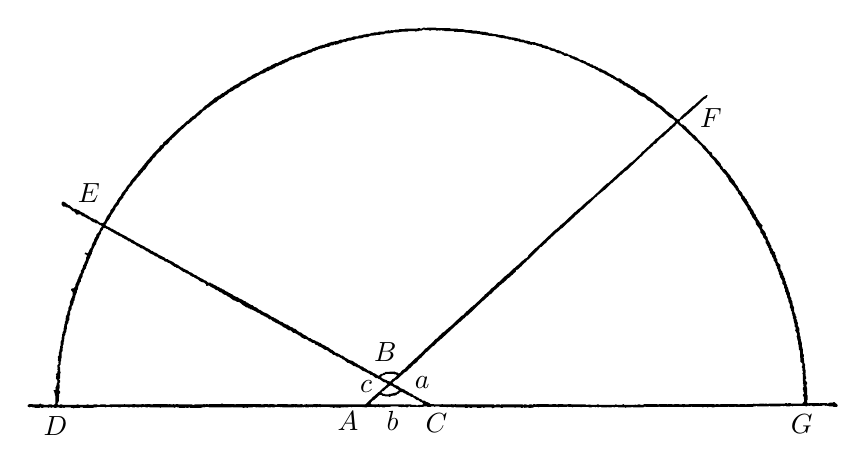
\begin{tikzpicture}[x=0.00607639cm,y=-0.00607639cm]
\fill[even odd rule] (21,803) -- (21,805) -- (22,806) -- (24,806) -- (25,807) -- (27,806) -- (30,806) -- (31,807) -- (35,807) -- (36,808) -- (46,808) -- (47,807) -- (49,807) -- (50,808) -- (53,808) -- (54,807) -- (63,807) -- (64,808) -- (66,807) -- (69,807) -- (70,808) -- (72,807) -- (76,807) -- (77,808) -- (81,808) -- (82,807) -- (87,807) -- (88,808) -- (93,808) -- (94,807) -- (96,808) -- (98,808) -- (99,807) -- (111,807) -- (112,808) -- (115,808) -- (116,809) -- (118,809) -- (119,808) -- (130,808) -- (131,807) -- (136,807) -- (137,808) -- (158,808) -- (159,807) -- (165,807) -- (166,806) -- (182,806) -- (183,807) -- (185,807) -- (186,806) -- (194,806) -- (195,807) -- (197,807) -- (198,806) -- (210,806) -- (211,807) -- (215,807) -- (216,806) -- (230,806) -- (231,807) -- (234,807) -- (235,806) -- (239,806) -- (240,807) -- (245,807) -- (246,806) -- (248,806) -- (249,807) -- (254,807) -- (255,806) -- (257,806) -- (258,807) -- (260,807) -- (261,806) -- (267,806) -- (268,807) -- (272,807) -- (273,806) -- (275,806) -- (276,807) -- (297,807) -- (298,808) -- (300,807) -- (326,807) -- (328,808) -- (332,806) -- (334,807) -- (337,807) -- (338,808) -- (350,808) -- (351,807) -- (353,808) -- (357,808) -- (358,807) -- (360,807) -- (361,808) -- (384,808) -- (385,807) -- (388,807) -- (389,806) -- (391,807) -- (393,806) -- (399,806) -- (400,807) -- (447,807) -- (449,806) -- (450,807) -- (470,807) -- (471,808) -- (474,808) -- (475,807) -- (481,808) -- (482,807) -- (491,807) -- (492,806) -- (497,806) -- (498,807) -- (501,807) -- (502,806) -- (504,807) -- (517,807) -- (518,806) -- (522,806) -- (523,807) -- (530,807) -- (531,806) -- (533,807) -- (537,807) -- (538,806) -- (549,806) -- (550,807) -- (552,806) -- (554,807) -- (577,807) -- (578,806) -- (580,807) -- (582,807) -- (583,806) -- (585,807) -- (594,807) -- (595,806) -- (597,807) -- (599,806) -- (601,806) -- (602,807) -- (609,807) -- (610,806) -- (612,806) -- (613,807) -- (615,806) -- (617,807) -- (619,806) -- (626,807) -- (627,806) -- (631,806) -- (633,807) -- (634,806) -- (652,806) -- (653,807) -- (659,807) -- (660,808) -- (662,808) -- (663,807) -- (675,808) -- (676,807) -- (683,807) -- (684,806) -- (686,807) -- (691,807) -- (692,806) -- (697,806) -- (698,807) -- (700,806) -- (721,806) -- (722,807) -- (724,806) -- (726,807) -- (730,807) -- (731,806) -- (746,806) -- (747,807) -- (749,807) -- (750,806) -- (755,806) -- (756,807) -- (758,806) -- (762,806) -- (763,807) -- (768,807) -- (769,806) -- (779,806) -- (780,805) -- (796,805) -- (797,806) -- (802,806) -- (803,807) -- (805,806) -- (812,806) -- (813,807) -- (815,807) -- (818,805) -- (820,805) -- (821,806) -- (838,806) -- (840,807) -- (841,806) -- (848,806) -- (849,805) -- (856,805) -- (857,806) -- (864,806) -- (865,805) -- (871,805) -- (872,806) -- (874,805) -- (882,805) -- (883,806) -- (897,806) -- (898,807) -- (900,806) -- (907,806) -- (908,807) -- (912,807) -- (913,806) -- (915,806) -- (916,807) -- (935,807) -- (936,808) -- (941,808) -- (942,807) -- (945,807) -- (946,808) -- (950,808) -- (951,807) -- (960,807) -- (961,808) -- (969,808) -- (970,807) -- (973,807) -- (974,808) -- (976,808) -- (977,807) -- (991,807) -- (993,809) -- (998,807) -- (1010,807) -- (1011,808) -- (1014,808) -- (1015,807) -- (1039,807) -- (1040,808) -- (1042,807) -- (1052,807) -- (1053,808) -- (1056,808) -- (1057,807) -- (1059,807) -- (1060,808) -- (1068,807) -- (1069,808) -- (1074,808) -- (1076,807) -- (1077,808) -- (1080,806) -- (1088,806) -- (1089,807) -- (1091,806) -- (1129,806) -- (1131,807) -- (1132,806) -- (1149,806) -- (1150,805) -- (1152,806) -- (1159,806) -- (1160,807) -- (1162,806) -- (1177,806) -- (1178,807) -- (1180,806) -- (1194,806) -- (1195,807) -- (1200,807) -- (1201,806) -- (1207,806) -- (1208,807) -- (1210,806) -- (1212,806) -- (1213,807) -- (1215,807) -- (1216,806) -- (1220,806) -- (1221,807) -- (1233,807) -- (1234,806) -- (1236,807) -- (1242,807) -- (1243,806) -- (1249,807) -- (1250,806) -- (1255,806) -- (1256,807) -- (1270,807) -- (1272,808) -- (1273,807) -- (1283,807) -- (1284,806) -- (1286,806) -- (1287,807) -- (1308,807) -- (1312,805) -- (1314,806) -- (1340,806) -- (1341,805) -- (1343,806) -- (1392,806) -- (1393,807) -- (1395,806) -- (1408,806) -- (1410,805) -- (1411,806) -- (1431,806) -- (1432,807) -- (1434,807) -- (1435,806) -- (1441,806) -- (1442,807) -- (1444,807) -- (1445,806) -- (1451,806) -- (1452,807) -- (1457,807) -- (1458,806) -- (1485,806) -- (1486,805) -- (1488,806) -- (1499,806) -- (1500,805) -- (1502,806) -- (1538,806) -- (1539,805) -- (1543,805) -- (1544,804) -- (1546,804) -- (1547,805) -- (1570,805) -- (1571,804) -- (1573,804) -- (1574,805) -- (1595,805) -- (1596,804) -- (1601,804) -- (1602,805) -- (1604,804) -- (1607,804) -- (1608,805) -- (1615,805) -- (1616,804) -- (1619,804) -- (1620,805) -- (1622,804) -- (1647,804) -- (1648,805) -- (1650,805) -- (1653,803) -- (1655,804) -- (1661,803) -- (1662,804) -- (1666,805) -- (1667,804) -- (1682,804) -- (1683,803) -- (1688,803) -- (1690,804) -- (1692,803) -- (1693,804) -- (1696,804) -- (1697,805) -- (1705,805) -- (1706,806) -- (1713,806) -- (1715,804) -- (1715,802) -- (1708,796) -- (1706,796) -- (1705,797) -- (1699,797) -- (1695,799) -- (1693,799) -- (1692,798) -- (1678,798) -- (1677,799) -- (1675,798) -- (1655,798) -- (1653,799) -- (1651,797) -- (1651,792) -- (1652,791) -- (1652,782) -- (1651,781) -- (1651,766) -- (1650,765) -- (1650,762) -- (1649,761) -- (1649,760) -- (1651,758) -- (1651,755) -- (1647,750) -- (1647,749) -- (1649,747) -- (1649,743) -- (1648,742) -- (1648,738) -- (1647,737) -- (1648,735) -- (1648,729) -- (1647,728) -- (1647,724) -- (1646,723) -- (1647,718) -- (1645,714) -- (1644,704) -- (1643,703) -- (1644,701) -- (1644,697) -- (1642,694) -- (1642,685) -- (1641,684) -- (1641,681) -- (1640,680) -- (1640,672) -- (1639,671) -- (1639,668) -- (1638,667) -- (1637,658) -- (1635,656) -- (1636,654) -- (1635,650) -- (1634,649) -- (1635,647) -- (1635,643) -- (1631,635) -- (1632,631) -- (1630,627) -- (1630,624) -- (1628,622) -- (1629,618) -- (1627,616) -- (1627,613) -- (1624,607) -- (1624,603) -- (1623,602) -- (1624,599) -- (1621,593) -- (1620,585) -- (1618,582) -- (1618,578) -- (1616,576) -- (1616,574) -- (1615,573) -- (1615,568) -- (1613,565) -- (1611,557) -- (1609,554) -- (1609,551) -- (1607,549) -- (1607,545) -- (1605,542) -- (1605,538) -- (1603,535) -- (1603,533) -- (1601,531) -- (1601,527) -- (1599,525) -- (1599,523) -- (1597,521) -- (1595,517) -- (1595,509) -- (1590,504) -- (1589,502) -- (1589,498) -- (1586,494) -- (1586,490) -- (1584,487) -- (1584,483) -- (1580,480) -- (1579,476) -- (1576,473) -- (1576,469) -- (1574,467) -- (1574,465) -- (1569,456) -- (1568,451) -- (1565,448) -- (1565,444) -- (1563,440) -- (1557,433) -- (1557,429) -- (1558,427) -- (1552,421) -- (1551,418) -- (1547,413) -- (1547,411) -- (1544,408) -- (1544,405) -- (1541,402) -- (1538,395) -- (1534,390) -- (1533,387) -- (1528,381) -- (1528,378) -- (1525,375) -- (1525,373) -- (1521,369) -- (1521,367) -- (1516,363) -- (1516,361) -- (1514,357) -- (1509,352) -- (1506,345) -- (1501,339) -- (1499,334) -- (1492,326) -- (1491,323) -- (1483,314) -- (1483,313) -- (1479,309) -- (1477,309) -- (1475,307) -- (1474,304) -- (1471,301) -- (1470,297) -- (1462,288) -- (1462,287) -- (1453,280) -- (1452,275) -- (1450,273) -- (1447,272) -- (1444,269) -- (1444,268) -- (1440,264) -- (1440,263) -- (1436,259) -- (1435,259) -- (1427,251) -- (1426,249) -- (1425,249) -- (1422,246) -- (1422,245) -- (1416,238) -- (1412,236) -- (1405,229) -- (1405,228) -- (1399,223) -- (1399,222) -- (1396,219) -- (1395,219) -- (1392,216) -- (1388,215) -- (1384,210) -- (1385,207) -- (1387,205) -- (1390,204) -- (1395,199) -- (1396,199) -- (1401,194) -- (1402,194) -- (1408,188) -- (1409,188) -- (1414,182) -- (1416,182) -- (1417,180) -- (1420,177) -- (1421,177) -- (1436,162) -- (1439,161) -- (1441,159) -- (1443,154) -- (1440,154) -- (1438,156) -- (1434,158) -- (1421,170) -- (1420,170) -- (1416,175) -- (1412,177) -- (1396,192) -- (1395,192) -- (1386,201) -- (1386,202) -- (1384,204) -- (1380,205) -- (1375,201) -- (1374,201) -- (1370,196) -- (1369,196) -- (1366,193) -- (1365,193) -- (1362,190) -- (1357,187) -- (1355,185) -- (1355,184) -- (1347,177) -- (1341,174) -- (1335,168) -- (1332,167) -- (1324,160) -- (1317,156) -- (1310,150) -- (1303,148) -- (1296,142) -- (1293,141) -- (1289,137) -- (1287,137) -- (1285,135) -- (1283,135) -- (1280,132) -- (1277,131) -- (1275,129) -- (1271,128) -- (1268,125) -- (1265,124) -- (1261,120) -- (1259,119) -- (1254,119) -- (1246,113) -- (1236,108) -- (1229,103) -- (1225,102) -- (1218,98) -- (1215,98) -- (1212,95) -- (1210,95) -- (1208,93) -- (1205,93) -- (1202,90) -- (1198,90) -- (1195,87) -- (1193,87) -- (1189,85) -- (1187,83) -- (1185,83) -- (1182,81) -- (1176,80) -- (1169,75) -- (1167,75) -- (1164,73) -- (1161,73) -- (1158,71) -- (1151,69) -- (1149,67) -- (1144,67) -- (1141,64) -- (1139,64) -- (1134,61) -- (1132,61) -- (1131,60) -- (1127,60) -- (1123,57) -- (1117,56) -- (1114,54) -- (1111,54) -- (1107,51) -- (1100,50) -- (1095,47) -- (1090,47) -- (1089,46) -- (1084,45) -- (1081,43) -- (1073,43) -- (1070,41) -- (1067,41) -- (1066,40) -- (1061,40) -- (1057,38) -- (1052,38) -- (1050,36) -- (1046,36) -- (1045,35) -- (1042,35) -- (1041,34) -- (1031,33) -- (1030,32) -- (1027,32) -- (1026,31) -- (1021,31) -- (1017,29) -- (1005,28) -- (1004,27) -- (993,26) -- (992,25) -- (986,25) -- (983,23) -- (980,23) -- (979,22) -- (973,22) -- (972,21) -- (967,21) -- (966,20) -- (961,20) -- (960,19) -- (951,19) -- (950,18) -- (937,18) -- (936,17) -- (933,17) -- (932,16) -- (921,16) -- (920,15) -- (905,15) -- (904,14) -- (876,14) -- (875,13) -- (856,13) -- (855,14) -- (853,14) -- (852,13) -- (848,13) -- (845,15) -- (842,15) -- (841,14) -- (837,14) -- (836,15) -- (810,15) -- (809,16) -- (798,16) -- (797,17) -- (790,17) -- (789,18) -- (786,18) -- (785,19) -- (783,18) -- (781,18) -- (780,19) -- (777,19) -- (775,18) -- (774,19) -- (770,19) -- (767,21) -- (756,21) -- (753,23) -- (745,23) -- (744,24) -- (740,24) -- (736,26) -- (729,26) -- (728,27) -- (724,27) -- (723,28) -- (720,28) -- (719,29) -- (714,29) -- (712,31) -- (703,31) -- (697,34) -- (692,34) -- (691,35) -- (688,35) -- (685,37) -- (682,37) -- (681,38) -- (675,38) -- (669,41) -- (664,41) -- (663,42) -- (655,43) -- (654,44) -- (649,45) -- (647,47) -- (644,47) -- (641,49) -- (637,49) -- (636,50) -- (634,50) -- (627,53) -- (624,53) -- (621,55) -- (617,56) -- (615,58) -- (607,60) -- (605,62) -- (599,63) -- (598,64) -- (595,64) -- (591,67) -- (585,68) -- (582,70) -- (580,70) -- (576,73) -- (572,73) -- (563,78) -- (561,78) -- (555,81) -- (553,81) -- (551,83) -- (546,85) -- (544,87) -- (540,87) -- (530,92) -- (528,94) -- (523,95) -- (519,98) -- (515,99) -- (512,102) -- (507,104) -- (505,106) -- (501,108) -- (499,108) -- (491,112) -- (486,116) -- (484,116) -- (477,121) -- (471,124) -- (467,125) -- (463,129) -- (451,135) -- (448,138) -- (446,138) -- (442,142) -- (440,142) -- (436,146) -- (435,146) -- (430,150) -- (428,150) -- (422,155) -- (420,155) -- (415,159) -- (413,159) -- (406,166) -- (405,166) -- (396,174) -- (392,176) -- (385,184) -- (382,185) -- (369,197) -- (366,198) -- (363,201) -- (362,201) -- (357,207) -- (353,209) -- (345,217) -- (344,217) -- (338,223) -- (337,223) -- (308,251) -- (307,251) -- (304,254) -- (304,256) -- (302,258) -- (299,259) -- (297,261) -- (296,264) -- (282,278) -- (282,279) -- (276,285) -- (276,286) -- (269,293) -- (269,294) -- (265,298) -- (265,299) -- (261,303) -- (261,304) -- (257,308) -- (257,309) -- (252,314) -- (251,317) -- (237,333) -- (234,339) -- (229,344) -- (225,351) -- (218,359) -- (216,364) -- (210,371) -- (210,372) -- (208,374) -- (208,376) -- (201,385) -- (198,391) -- (194,395) -- (194,397) -- (192,401) -- (187,407) -- (182,418) -- (178,422) -- (176,421) -- (172,421) -- (165,415) -- (163,414) -- (160,414) -- (158,412) -- (154,411) -- (144,404) -- (142,404) -- (139,401) -- (132,398) -- (130,396) -- (126,394) -- (124,394) -- (122,392) -- (118,392) -- (116,391) -- (108,384) -- (106,384) -- (100,379) -- (96,377) -- (94,377) -- (92,379) -- (92,383) -- (95,387) -- (100,387) -- (102,389) -- (105,389) -- (109,391) -- (115,397) -- (118,397) -- (123,404) -- (131,403) -- (135,407) -- (139,408) -- (149,414) -- (151,414) -- (155,418) -- (159,420) -- (161,420) -- (163,422) -- (167,422) -- (172,426) -- (174,426) -- (176,428) -- (176,429) -- (172,434) -- (172,436) -- (170,440) -- (165,445) -- (164,450) -- (162,452) -- (160,456) -- (160,458) -- (156,465) -- (154,473) -- (151,476) -- (148,483) -- (146,485) -- (142,483) -- (140,486) -- (141,487) -- (143,487) -- (145,489) -- (145,491) -- (143,494) -- (143,498) -- (142,499) -- (142,501) -- (140,504) -- (139,508) -- (137,510) -- (136,515) -- (134,519) -- (132,521) -- (132,526) -- (129,530) -- (129,532) -- (127,535) -- (127,537) -- (125,540) -- (125,542) -- (121,550) -- (121,553) -- (120,555) -- (117,558) -- (114,558) -- (112,560) -- (112,562) -- (115,566) -- (115,573) -- (109,587) -- (109,593) -- (106,599) -- (106,604) -- (104,607) -- (104,611) -- (103,612) -- (103,614) -- (101,616) -- (100,627) -- (99,628) -- (99,632) -- (98,633) -- (98,636) -- (97,637) -- (97,640) -- (96,641) -- (96,647) -- (94,650) -- (94,653) -- (93,654) -- (93,660) -- (92,661) -- (92,666) -- (90,670) -- (90,678) -- (89,679) -- (89,684) -- (88,685) -- (87,691) -- (86,692) -- (86,699) -- (84,701) -- (84,703) -- (85,704) -- (84,709) -- (86,711) -- (85,713) -- (86,716) -- (83,719) -- (83,723) -- (84,724) -- (83,728) -- (84,729) -- (84,731) -- (83,732) -- (83,735) -- (80,738) -- (81,740) -- (80,746) -- (83,751) -- (83,755) -- (82,756) -- (81,762) -- (79,766) -- (80,769) -- (78,771) -- (76,771) -- (75,772) -- (77,775) -- (77,777) -- (78,778) -- (78,782) -- (79,783) -- (79,799) -- (76,802) -- (72,802) -- (71,801) -- (65,801) -- (64,802) -- (55,802) -- (54,801) -- (50,801) -- (48,799) -- (47,799) -- (44,801) -- (32,801) -- (31,800) -- (24,800) -- cycle
(848,800) -- (846,802) -- (838,802) -- (837,803) -- (834,803) -- (833,802) -- (824,802) -- (823,801) -- (811,801) -- (810,802) -- (808,801) -- (756,801) -- (755,800) -- (753,801) -- (740,801) -- (738,799) -- (738,798) -- (742,793) -- (746,791) -- (757,781) -- (761,781) -- (763,783) -- (767,783) -- (768,784) -- (776,784) -- (777,785) -- (779,785) -- (781,783) -- (791,782) -- (794,779) -- (796,779) -- (800,775) -- (805,775) -- (809,778) -- (811,778) -- (813,780) -- (817,782) -- (819,782) -- (823,785) -- (826,785) -- (835,792) -- (838,792) -- (843,796) -- (845,796) -- (848,799) -- cycle
(797,771) -- (797,772) -- (792,776) -- (786,777) -- (785,778) -- (782,778) -- (781,779) -- (777,779) -- (776,780) -- (769,780) -- (768,779) -- (765,779) -- (761,776) -- (761,775) -- (763,773) -- (765,773) -- (771,767) -- (772,767) -- (776,763) -- (780,761) -- (785,763) -- (787,765) -- (790,766) -- (793,769) -- (795,769) -- cycle
(760,744) -- (760,743) -- (763,740) -- (768,739) -- (770,737) -- (787,737) -- (788,738) -- (791,738) -- (793,740) -- (793,741) -- (788,746) -- (784,748) -- (780,753) -- (774,752) -- (772,750) -- (768,749) -- (762,746) -- cycle
(83,800) -- (86,794) -- (86,786) -- (87,785) -- (87,782) -- (86,780) -- (89,777) -- (89,774) -- (87,772) -- (87,768) -- (88,767) -- (88,760) -- (87,759) -- (87,757) -- (89,754) -- (89,751) -- (87,749) -- (87,748) -- (89,746) -- (89,736) -- (90,735) -- (90,733) -- (89,732) -- (89,724) -- (88,723) -- (88,720) -- (90,717) -- (90,711) -- (91,710) -- (91,705) -- (92,704) -- (92,692) -- (94,689) -- (94,683) -- (95,682) -- (94,679) -- (96,675) -- (96,670) -- (97,669) -- (98,658) -- (100,655) -- (100,652) -- (102,648) -- (102,644) -- (103,643) -- (103,635) -- (106,630) -- (106,627) -- (108,624) -- (108,616) -- (110,613) -- (110,606) -- (113,601) -- (113,596) -- (116,592) -- (116,590) -- (117,589) -- (117,585) -- (119,583) -- (119,579) -- (120,578) -- (120,576) -- (121,575) -- (121,573) -- (124,566) -- (124,563) -- (126,560) -- (127,553) -- (129,550) -- (130,546) -- (132,544) -- (132,539) -- (134,537) -- (136,533) -- (136,529) -- (139,524) -- (139,521) -- (143,516) -- (143,513) -- (145,510) -- (145,508) -- (147,505) -- (149,498) -- (152,493) -- (152,491) -- (155,486) -- (155,483) -- (157,481) -- (157,478) -- (162,468) -- (164,466) -- (165,461) -- (171,450) -- (171,448) -- (174,444) -- (175,439) -- (178,436) -- (178,434) -- (180,432) -- (184,432) -- (186,434) -- (188,434) -- (191,437) -- (193,437) -- (197,440) -- (200,441) -- (202,443) -- (205,444) -- (207,446) -- (209,446) -- (211,448) -- (217,450) -- (220,453) -- (222,453) -- (224,455) -- (229,457) -- (232,460) -- (235,460) -- (238,463) -- (247,467) -- (250,470) -- (254,471) -- (257,474) -- (262,475) -- (264,477) -- (265,477) -- (270,481) -- (272,481) -- (277,485) -- (284,488) -- (288,491) -- (292,492) -- (295,495) -- (305,499) -- (308,502) -- (311,502) -- (315,505) -- (317,505) -- (328,513) -- (330,513) -- (332,515) -- (336,516) -- (347,524) -- (350,524) -- (353,527) -- (355,527) -- (359,529) -- (362,532) -- (366,534) -- (368,534) -- (370,536) -- (378,540) -- (381,543) -- (385,545) -- (390,546) -- (394,550) -- (394,552) -- (395,553) -- (397,553) -- (398,552) -- (402,553) -- (404,555) -- (412,559) -- (415,562) -- (418,562) -- (423,566) -- (427,567) -- (430,570) -- (434,572) -- (436,572) -- (439,575) -- (442,576) -- (451,583) -- (455,584) -- (458,586) -- (464,587) -- (472,594) -- (473,594) -- (478,598) -- (481,598) -- (483,600) -- (485,600) -- (487,602) -- (489,602) -- (499,607) -- (501,609) -- (503,609) -- (507,611) -- (509,613) -- (514,615) -- (516,617) -- (518,617) -- (520,619) -- (522,619) -- (526,623) -- (530,623) -- (534,627) -- (537,628) -- (541,631) -- (543,631) -- (545,633) -- (547,633) -- (549,635) -- (552,636) -- (555,639) -- (560,641) -- (567,646) -- (571,646) -- (576,651) -- (579,651) -- (585,654) -- (587,656) -- (590,657) -- (594,661) -- (600,664) -- (603,664) -- (607,666) -- (610,669) -- (612,669) -- (616,672) -- (620,672) -- (623,676) -- (627,677) -- (630,680) -- (632,680) -- (636,682) -- (643,687) -- (646,687) -- (648,688) -- (654,693) -- (656,693) -- (660,697) -- (663,697) -- (668,701) -- (672,701) -- (674,703) -- (677,704) -- (680,707) -- (682,707) -- (690,714) -- (692,714) -- (698,717) -- (703,721) -- (706,721) -- (709,723) -- (713,724) -- (722,731) -- (724,731) -- (736,737) -- (738,739) -- (741,739) -- (749,746) -- (753,746) -- (755,748) -- (757,748) -- (765,754) -- (770,755) -- (773,758) -- (773,759) -- (766,766) -- (765,766) -- (756,775) -- (755,775) -- (745,784) -- (744,784) -- (738,791) -- (737,791) -- (728,800) -- (726,801) -- (634,801) -- (633,800) -- (630,800) -- (629,801) -- (627,800) -- (619,800) -- (618,801) -- (606,801) -- (604,800) -- (603,801) -- (600,801) -- (598,802) -- (594,800) -- (592,800) -- (591,801) -- (585,801) -- (584,800) -- (580,800) -- (579,801) -- (577,800) -- (573,800) -- (572,801) -- (565,801) -- (564,800) -- (544,800) -- (540,802) -- (539,801) -- (536,801) -- (535,800) -- (527,800) -- (526,801) -- (524,801) -- (523,800) -- (515,800) -- (514,801) -- (509,801) -- (508,800) -- (457,800) -- (456,801) -- (454,801) -- (453,800) -- (430,800) -- (429,799) -- (426,799) -- (425,800) -- (401,800) -- (400,801) -- (398,801) -- (397,800) -- (394,800) -- (393,801) -- (389,800) -- (388,801) -- (370,801) -- (369,802) -- (366,802) -- (365,801) -- (336,801) -- (335,800) -- (332,800) -- (331,801) -- (327,801) -- (326,800) -- (324,801) -- (320,801) -- (319,800) -- (317,800) -- (316,801) -- (314,801) -- (313,800) -- (284,800) -- (283,801) -- (278,801) -- (277,800) -- (271,800) -- (270,801) -- (268,800) -- (266,801) -- (264,801) -- (263,800) -- (260,800) -- (259,801) -- (246,801) -- (245,800) -- (241,800) -- (240,801) -- (225,801) -- (223,800) -- (222,801) -- (193,801) -- (192,802) -- (185,802) -- (184,801) -- (173,801) -- (172,802) -- (167,802) -- (166,801) -- (159,801) -- (158,802) -- (149,802) -- (148,801) -- (145,801) -- (144,802) -- (128,802) -- (127,801) -- (124,801) -- (123,802) -- (94,802) -- (93,801) -- (89,801) -- (88,802) -- (85,802) -- cycle
(1645,794) -- (1641,799) -- (1617,799) -- (1616,798) -- (1612,798) -- (1611,799) -- (1609,799) -- (1608,798) -- (1606,798) -- (1605,799) -- (1571,799) -- (1570,800) -- (1568,800) -- (1567,799) -- (1563,799) -- (1562,800) -- (1560,799) -- (1541,800) -- (1539,799) -- (1538,800) -- (1525,800) -- (1524,801) -- (1522,801) -- (1521,800) -- (1511,800) -- (1510,801) -- (1506,801) -- (1505,800) -- (1470,800) -- (1469,801) -- (1466,801) -- (1465,800) -- (1461,800) -- (1460,801) -- (1457,801) -- (1456,800) -- (1404,800) -- (1403,801) -- (1396,801) -- (1395,800) -- (1390,800) -- (1389,801) -- (1384,801) -- (1383,800) -- (1374,800) -- (1373,801) -- (1369,801) -- (1368,800) -- (1361,800) -- (1360,801) -- (1358,800) -- (1342,800) -- (1341,801) -- (1338,801) -- (1337,800) -- (1310,800) -- (1308,802) -- (1303,802) -- (1302,801) -- (1297,801) -- (1296,802) -- (1293,802) -- (1292,801) -- (1290,802) -- (1269,802) -- (1267,800) -- (1266,800) -- (1264,802) -- (1253,802) -- (1252,801) -- (1250,801) -- (1249,802) -- (1216,802) -- (1215,801) -- (1212,801) -- (1211,802) -- (1198,802) -- (1197,801) -- (1189,802) -- (1188,801) -- (1158,801) -- (1157,800) -- (1151,800) -- (1150,801) -- (1141,801) -- (1140,800) -- (1131,800) -- (1130,801) -- (1126,801) -- (1125,800) -- (1119,800) -- (1118,801) -- (1111,801) -- (1110,800) -- (1086,800) -- (1085,801) -- (1082,801) -- (1081,800) -- (1079,800) -- (1077,802) -- (1075,801) -- (1070,801) -- (1069,802) -- (1065,802) -- (1064,801) -- (1059,801) -- (1058,802) -- (1056,801) -- (1011,801) -- (1010,802) -- (1008,801) -- (1001,801) -- (1000,802) -- (997,802) -- (996,801) -- (939,801) -- (938,800) -- (936,801) -- (917,801) -- (916,800) -- (914,801) -- (909,801) -- (908,800) -- (906,801) -- (890,801) -- (889,800) -- (887,800) -- (886,801) -- (871,801) -- (870,800) -- (863,800) -- (861,798) -- (857,796) -- (855,796) -- (851,793) -- (847,793) -- (844,790) -- (840,789) -- (837,786) -- (835,786) -- (833,784) -- (829,783) -- (825,779) -- (823,778) -- (820,778) -- (817,775) -- (816,775) -- (814,773) -- (812,773) -- (809,770) -- (801,767) -- (795,762) -- (788,760) -- (784,756) -- (784,755) -- (791,749) -- (793,749) -- (809,734) -- (815,731) -- (816,729) -- (820,725) -- (821,725) -- (828,717) -- (833,714) -- (837,710) -- (837,709) -- (842,704) -- (843,704) -- (855,691) -- (856,691) -- (867,680) -- (871,678) -- (879,669) -- (880,669) -- (885,664) -- (886,664) -- (917,635) -- (918,635) -- (925,628) -- (926,628) -- (933,621) -- (934,621) -- (939,615) -- (941,615) -- (973,584) -- (974,584) -- (982,576) -- (983,576) -- (987,571) -- (990,570) -- (998,561) -- (999,561) -- (1004,556) -- (1005,556) -- (1009,551) -- (1010,551) -- (1014,547) -- (1015,547) -- (1019,543) -- (1020,543) -- (1025,537) -- (1029,535) -- (1034,530) -- (1035,530) -- (1036,528) -- (1042,523) -- (1042,521) -- (1044,519) -- (1046,519) -- (1053,512) -- (1054,512) -- (1055,510) -- (1061,504) -- (1062,504) -- (1064,502) -- (1064,501) -- (1067,498) -- (1068,498) -- (1091,475) -- (1091,474) -- (1093,472) -- (1096,471) -- (1103,464) -- (1104,464) -- (1106,462) -- (1106,461) -- (1112,455) -- (1113,455) -- (1117,450) -- (1118,450) -- (1127,441) -- (1128,441) -- (1138,432) -- (1139,432) -- (1151,420) -- (1152,420) -- (1160,412) -- (1161,412) -- (1168,404) -- (1169,404) -- (1173,400) -- (1174,400) -- (1178,395) -- (1183,392) -- (1194,381) -- (1195,381) -- (1209,367) -- (1210,367) -- (1214,362) -- (1215,362) -- (1227,352) -- (1228,352) -- (1242,338) -- (1243,338) -- (1250,331) -- (1251,331) -- (1261,321) -- (1262,321) -- (1269,314) -- (1274,311) -- (1298,288) -- (1299,288) -- (1300,286) -- (1303,283) -- (1304,283) -- (1313,273) -- (1314,273) -- (1321,266) -- (1322,266) -- (1327,261) -- (1328,261) -- (1330,257) -- (1335,255) -- (1337,253) -- (1337,252) -- (1346,243) -- (1350,241) -- (1360,231) -- (1361,231) -- (1365,226) -- (1366,226) -- (1372,220) -- (1373,220) -- (1376,217) -- (1376,216) -- (1379,213) -- (1380,213) -- (1386,219) -- (1387,219) -- (1393,226) -- (1394,226) -- (1405,237) -- (1406,237) -- (1417,249) -- (1420,250) -- (1422,252) -- (1422,253) -- (1430,260) -- (1433,265) -- (1442,274) -- (1442,275) -- (1446,278) -- (1447,281) -- (1456,290) -- (1461,298) -- (1468,305) -- (1469,308) -- (1474,313) -- (1474,314) -- (1482,322) -- (1482,324) -- (1485,327) -- (1488,334) -- (1498,345) -- (1498,346) -- (1501,349) -- (1502,352) -- (1506,356) -- (1507,360) -- (1513,367) -- (1513,370) -- (1526,389) -- (1527,393) -- (1530,396) -- (1532,400) -- (1532,402) -- (1534,404) -- (1536,409) -- (1543,418) -- (1544,424) -- (1551,433) -- (1553,437) -- (1553,441) -- (1556,444) -- (1559,449) -- (1559,451) -- (1564,457) -- (1564,463) -- (1566,465) -- (1567,468) -- (1569,470) -- (1569,472) -- (1571,474) -- (1571,477) -- (1573,480) -- (1573,482) -- (1575,486) -- (1577,488) -- (1578,492) -- (1581,497) -- (1581,500) -- (1583,502) -- (1585,506) -- (1585,509) -- (1588,513) -- (1588,516) -- (1590,519) -- (1590,521) -- (1592,525) -- (1592,528) -- (1594,531) -- (1594,534) -- (1599,542) -- (1599,548) -- (1603,553) -- (1603,557) -- (1605,561) -- (1605,565) -- (1607,567) -- (1607,570) -- (1609,573) -- (1609,576) -- (1612,582) -- (1612,586) -- (1615,592) -- (1615,599) -- (1617,601) -- (1617,604) -- (1619,607) -- (1619,611) -- (1620,612) -- (1620,615) -- (1621,616) -- (1621,620) -- (1623,623) -- (1623,627) -- (1624,628) -- (1624,631) -- (1625,632) -- (1625,638) -- (1627,640) -- (1627,644) -- (1626,646) -- (1630,653) -- (1630,657) -- (1629,658) -- (1629,660) -- (1630,661) -- (1631,667) -- (1632,668) -- (1632,675) -- (1633,676) -- (1634,686) -- (1636,688) -- (1637,712) -- (1641,715) -- (1641,720) -- (1640,721) -- (1640,724) -- (1642,726) -- (1641,728) -- (1641,730) -- (1642,731) -- (1642,735) -- (1641,736) -- (1642,738) -- (1642,752) -- (1643,753) -- (1642,757) -- (1643,758) -- (1643,762) -- (1644,763) -- (1644,764) -- (1642,766) -- (1642,770) -- (1643,771) -- (1643,774) -- (1644,775) -- (1644,779) -- (1642,781) -- (1642,782) -- (1644,785) -- cycle
(1375,208) -- (1375,210) -- (1366,219) -- (1365,219) -- (1360,225) -- (1359,225) -- (1354,230) -- (1353,230) -- (1338,244) -- (1334,246) -- (1333,248) -- (1326,255) -- (1325,255) -- (1318,263) -- (1317,263) -- (1309,271) -- (1308,271) -- (1304,275) -- (1304,276) -- (1285,294) -- (1281,296) -- (1272,305) -- (1271,305) -- (1264,312) -- (1263,312) -- (1235,338) -- (1232,339) -- (1202,368) -- (1201,368) -- (1197,372) -- (1196,372) -- (1192,376) -- (1191,376) -- (1174,392) -- (1173,392) -- (1167,398) -- (1166,398) -- (1142,421) -- (1141,421) -- (1137,425) -- (1136,425) -- (1131,431) -- (1130,431) -- (1126,435) -- (1125,435) -- (1084,474) -- (1083,474) -- (1068,489) -- (1067,492) -- (1064,495) -- (1061,496) -- (1057,500) -- (1056,500) -- (1046,510) -- (1045,510) -- (1039,516) -- (1038,516) -- (1026,528) -- (1025,528) -- (1021,532) -- (1020,532) -- (1007,545) -- (1005,545) -- (996,555) -- (991,558) -- (985,565) -- (984,565) -- (979,570) -- (978,570) -- (976,572) -- (976,573) -- (955,593) -- (954,593) -- (950,597) -- (949,597) -- (940,606) -- (939,606) -- (932,614) -- (928,616) -- (904,639) -- (903,639) -- (892,649) -- (888,651) -- (886,653) -- (886,654) -- (884,656) -- (883,656) -- (877,663) -- (874,664) -- (871,667) -- (871,668) -- (855,683) -- (854,683) -- (843,695) -- (842,695) -- (833,704) -- (832,704) -- (820,716) -- (819,716) -- (809,727) -- (805,729) -- (802,732) -- (802,733) -- (798,736) -- (796,736) -- (794,734) -- (792,734) -- (788,732) -- (769,733) -- (767,735) -- (765,735) -- (763,737) -- (760,737) -- (757,740) -- (754,741) -- (747,736) -- (743,735) -- (741,733) -- (735,730) -- (733,730) -- (728,726) -- (725,725) -- (722,722) -- (717,721) -- (715,719) -- (712,718) -- (709,715) -- (707,715) -- (705,713) -- (704,713) -- (701,710) -- (693,708) -- (689,705) -- (686,704) -- (680,699) -- (677,699) -- (673,696) -- (667,693) -- (665,693) -- (658,687) -- (655,686) -- (649,681) -- (647,681) -- (643,678) -- (636,675) -- (633,672) -- (631,672) -- (626,669) -- (624,669) -- (622,667) -- (618,666) -- (614,664) -- (612,662) -- (609,662) -- (603,657) -- (598,655) -- (592,650) -- (589,650) -- (587,648) -- (586,648) -- (581,643) -- (577,642) -- (575,640) -- (571,639) -- (564,634) -- (562,634) -- (556,631) -- (554,629) -- (548,627) -- (545,624) -- (542,623) -- (540,621) -- (538,621) -- (536,619) -- (532,618) -- (522,611) -- (514,608) -- (507,603) -- (505,603) -- (499,598) -- (495,597) -- (491,593) -- (489,593) -- (483,590) -- (481,588) -- (479,588) -- (476,585) -- (474,585) -- (470,582) -- (463,579) -- (461,577) -- (457,576) -- (451,573) -- (448,570) -- (446,570) -- (444,568) -- (442,568) -- (440,566) -- (435,564) -- (432,561) -- (428,560) -- (426,558) -- (424,558) -- (420,555) -- (418,555) -- (416,553) -- (409,550) -- (407,548) -- (405,548) -- (403,546) -- (398,546) -- (394,542) -- (390,541) -- (388,539) -- (381,536) -- (379,534) -- (377,534) -- (374,531) -- (370,530) -- (363,525) -- (359,524) -- (356,521) -- (347,517) -- (345,515) -- (343,515) -- (341,513) -- (340,513) -- (335,509) -- (330,507) -- (325,503) -- (316,499) -- (314,497) -- (310,497) -- (306,493) -- (304,493) -- (302,491) -- (295,488) -- (290,484) -- (286,483) -- (282,480) -- (280,480) -- (275,476) -- (268,473) -- (266,471) -- (260,468) -- (258,468) -- (256,466) -- (246,461) -- (241,457) -- (239,457) -- (237,455) -- (230,452) -- (228,450) -- (214,443) -- (212,441) -- (208,440) -- (206,438) -- (201,436) -- (199,434) -- (195,433) -- (193,431) -- (186,428) -- (184,426) -- (184,424) -- (186,422) -- (187,419) -- (192,413) -- (193,410) -- (195,408) -- (195,406) -- (204,393) -- (205,389) -- (211,383) -- (214,376) -- (221,368) -- (221,366) -- (225,361) -- (226,358) -- (231,353) -- (231,351) -- (233,349) -- (233,348) -- (239,342) -- (241,338) -- (248,331) -- (249,328) -- (257,320) -- (257,319) -- (262,314) -- (262,313) -- (267,309) -- (274,298) -- (280,292) -- (283,287) -- (285,285) -- (286,285) -- (290,280) -- (290,279) -- (297,272) -- (298,272) -- (303,266) -- (305,265) -- (306,262) -- (310,258) -- (313,257) -- (318,251) -- (318,250) -- (320,248) -- (321,248) -- (323,246) -- (323,245) -- (325,243) -- (326,243) -- (344,225) -- (345,225) -- (356,214) -- (358,214) -- (369,204) -- (372,203) -- (376,198) -- (381,195) -- (388,187) -- (392,185) -- (397,180) -- (399,180) -- (412,170) -- (415,169) -- (421,163) -- (424,162) -- (426,160) -- (432,157) -- (435,154) -- (438,153) -- (443,148) -- (450,145) -- (456,140) -- (458,140) -- (462,138) -- (469,132) -- (477,129) -- (481,125) -- (483,125) -- (487,122) -- (499,116) -- (501,114) -- (503,114) -- (505,112) -- (511,109) -- (513,109) -- (519,106) -- (521,104) -- (524,104) -- (528,101) -- (532,100) -- (534,98) -- (536,98) -- (541,94) -- (543,94) -- (548,91) -- (551,91) -- (555,88) -- (557,88) -- (559,86) -- (563,85) -- (569,81) -- (571,81) -- (574,79) -- (577,79) -- (581,76) -- (589,75) -- (597,70) -- (601,70) -- (609,66) -- (614,65) -- (618,62) -- (622,62) -- (624,60) -- (626,60) -- (629,58) -- (631,58) -- (632,57) -- (636,57) -- (639,55) -- (642,55) -- (645,53) -- (651,53) -- (655,50) -- (660,50) -- (662,48) -- (664,48) -- (665,49) -- (667,48) -- (670,48) -- (672,46) -- (676,46) -- (678,44) -- (680,44) -- (682,42) -- (686,43) -- (692,40) -- (697,40) -- (698,39) -- (705,38) -- (708,36) -- (720,35) -- (724,33) -- (732,33) -- (737,30) -- (749,29) -- (750,28) -- (758,28) -- (759,27) -- (765,27) -- (769,25) -- (779,25) -- (780,24) -- (784,24) -- (788,22) -- (790,23) -- (797,23) -- (798,22) -- (802,22) -- (803,21) -- (816,21) -- (817,20) -- (831,20) -- (832,21) -- (834,21) -- (835,20) -- (839,20) -- (840,19) -- (845,19) -- (848,17) -- (851,17) -- (852,18) -- (860,18) -- (861,19) -- (864,19) -- (865,18) -- (874,18) -- (875,19) -- (879,19) -- (881,18) -- (882,19) -- (884,19) -- (885,18) -- (887,18) -- (888,19) -- (892,19) -- (893,20) -- (912,20) -- (914,22) -- (916,22) -- (917,21) -- (919,22) -- (934,22) -- (935,23) -- (947,24) -- (948,25) -- (966,26) -- (967,27) -- (970,27) -- (971,28) -- (978,28) -- (979,29) -- (984,29) -- (985,30) -- (1000,31) -- (1002,33) -- (1006,33) -- (1007,34) -- (1010,34) -- (1011,35) -- (1018,35) -- (1019,36) -- (1024,36) -- (1028,38) -- (1034,38) -- (1035,39) -- (1038,39) -- (1040,41) -- (1047,41) -- (1050,43) -- (1059,44) -- (1060,45) -- (1065,46) -- (1068,48) -- (1072,48) -- (1073,49) -- (1075,49) -- (1076,48) -- (1078,48) -- (1079,49) -- (1083,49) -- (1086,51) -- (1089,51) -- (1090,52) -- (1095,53) -- (1097,55) -- (1100,55) -- (1104,57) -- (1111,58) -- (1115,61) -- (1122,62) -- (1129,66) -- (1131,66) -- (1132,67) -- (1136,67) -- (1144,72) -- (1150,72) -- (1154,74) -- (1157,77) -- (1159,77) -- (1167,81) -- (1172,82) -- (1181,87) -- (1183,87) -- (1189,90) -- (1191,92) -- (1195,93) -- (1197,95) -- (1199,95) -- (1201,97) -- (1204,97) -- (1206,98) -- (1208,100) -- (1215,103) -- (1218,106) -- (1223,107) -- (1227,109) -- (1229,111) -- (1231,111) -- (1233,113) -- (1240,116) -- (1242,118) -- (1244,118) -- (1247,121) -- (1249,121) -- (1253,124) -- (1256,125) -- (1260,129) -- (1264,130) -- (1268,134) -- (1271,134) -- (1276,138) -- (1281,140) -- (1284,143) -- (1287,144) -- (1290,147) -- (1294,149) -- (1298,153) -- (1306,157) -- (1308,157) -- (1313,160) -- (1317,165) -- (1322,167) -- (1324,169) -- (1330,172) -- (1336,178) -- (1342,181) -- (1363,200) -- (1371,204) -- cycle;
\node[inner sep=0pt] at (1450,203) {$F$};
\node[inner sep=0pt] at (149,358) {$E$};
\node[inner sep=0pt] at (769,692) {$B$};
\node[inner sep=0pt] at (846,755) {$a$};
\node[inner sep=0pt] at (729,764) {$c$};
\node[inner sep=0pt] at (691,836) {$A$};
\node[inner sep=0pt] at (784,835) {$b$};
\node[inner sep=0pt] at (876,840) {$C$};
\node[inner sep=0pt] at (1640,841) {$G$};
\node[inner sep=0pt] at (79,846) {$D$};
\end{tikzpicture}

\end{center}

\noindent nehme einen Radius $R$ so gross, dass $\dfrac{a}{R}$, $\dfrac{b}{R}$, $\dfrac{c}{R}$ kleiner als jede gegebene Grösse werden. Mit diesem Radius beschreibe man aus $C$ den Halbkreis $DEFG$.
